\begin{itemize}
    \item The goal of linear discriminant analysis (LDA) is to find a vector w that maximizes the separation between the classes after projection onto w.
    \item The Fisher LDA objective: \[ \operatorname*{max}_w J(w) = \frac{(m_1 - m_2)^2}{s_1^2 + s_2^2}\] 
    \item We solve the problem by using the eigenvalue–eigenvector equation, as below. \[(S^{-1}B)w = \lambda w \]
    Thus, if \(S^{-1}\) exists, then \(\lambda\) = J(w) is an eigenvalue, and w is an eigenvector of the matrix
    \(S^{-1}\) B. To maximize J(w) we look for the largest eigenvalue \(\lambda\), and the corresponding dominant eigenvector w specifies the best linear discriminant vector.
    \item The key difference between principal component analysis and LDA is that the former deals with unlabeled data and tries to maximize variance, whereas the latter deals with labeled data and tries to maximize the discrimination between the classes.
    \begin{figure}[H]
        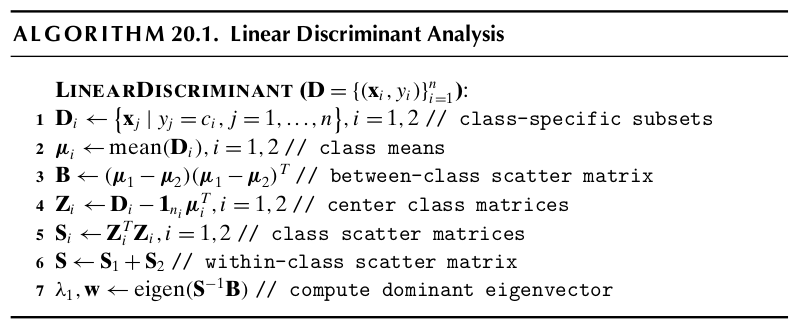
\includegraphics[width=\textwidth]{Figures/lda.png}
        \caption{\label{fig:figure2}LDA Algorithm, total time is
        O($d^3$ + $nd^2$).}
    \end{figure}
\end{itemize}